\section{Model inversion attack - images}
\label{sec:MIA}
In section ~\ref{sec:attackOnML}, we have discussed about the model inversion attack on machine learning systems. We showed images only for native Tensorflow trained model, and differentially private model with epsilon values 0.2 and 8 in section 6.5. The complete images we got from trained model with different epsilon values are shown in Figure A.1, A.2 and A.3.
\begin{figure}[h!]
     \begin{subfigure}{.325\textwidth}
         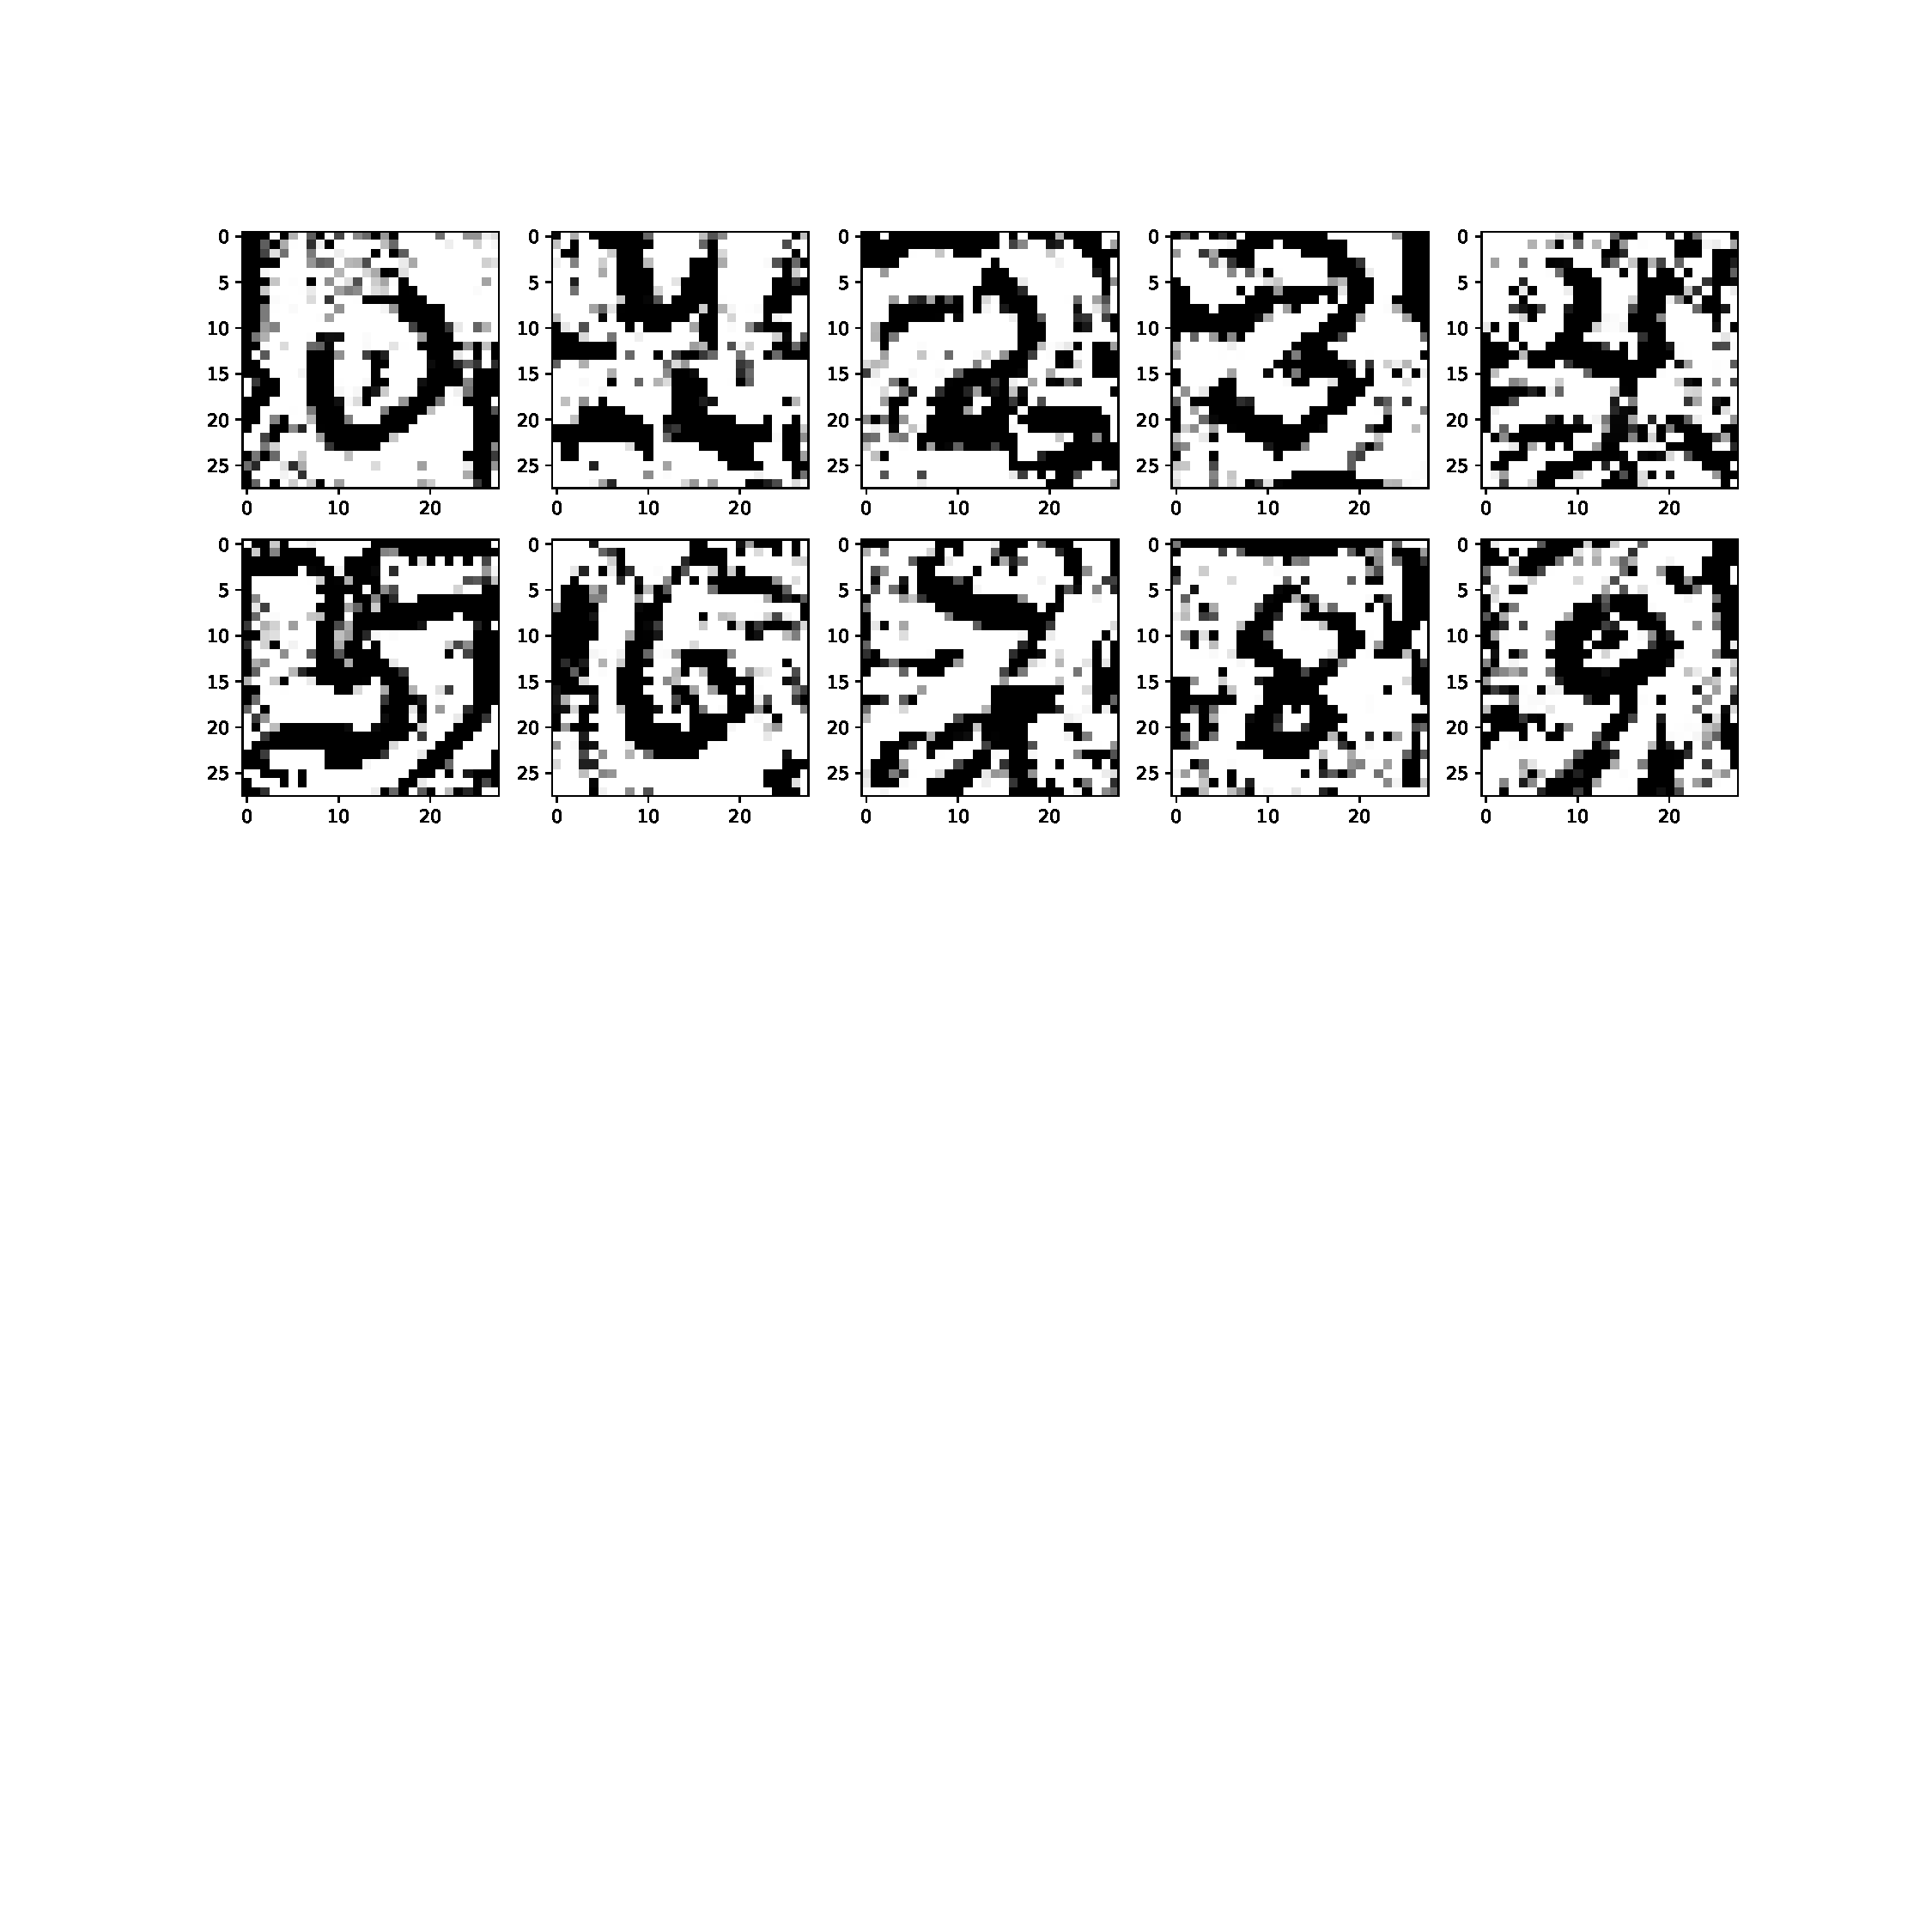
\includegraphics[width=\textwidth]{images/Native_attack/Mnistattack_native.pdf}
         \vspace{-8em}
         \caption{SPML+Native TensorFlow; and, Accuracy=99.55\%}
         \label{default}
     \end{subfigure}
     \begin{subfigure}{.325\textwidth}
         \includegraphics[width=\textwidth]{images/Native_attack/Mnistattack.2.pdf}
         \vspace{-8em}
         \caption{SPML+Privacy; $\epsilon$=0.2; and, Accuracy=10.12\%}
         \label{default}
     \end{subfigure}
     \begin{subfigure}{.325\textwidth}
         \includegraphics[width=\textwidth]{images/Native_attack/Mnistattack1.pdf}
         \vspace{-8em}
         \caption{SPML+Privacy; $\epsilon$=1 ; and, Accuracy=10.91\%}
         \label{default}
     \end{subfigure}
     \begin{subfigure}{.325\textwidth}
         \includegraphics[width=\textwidth]{images/Native_attack/Mnistattack2.pdf}
         \vspace{-8em}
         \caption{SPML+Privacy; $\epsilon$=2 ; and, Accuracy=10.63\%}
         \label{default}
     \end{subfigure}
     \begin{subfigure}{.325\textwidth}
         \includegraphics[width=\textwidth]{images/Native_attack/Mnistattack4.pdf}
         \vspace{-8em}
         \caption{SPML+Privacy; $\epsilon$=4 ; and, Accuracy=66.3\%}
         \label{default}
     \end{subfigure}
     \begin{subfigure}{.325\textwidth}
         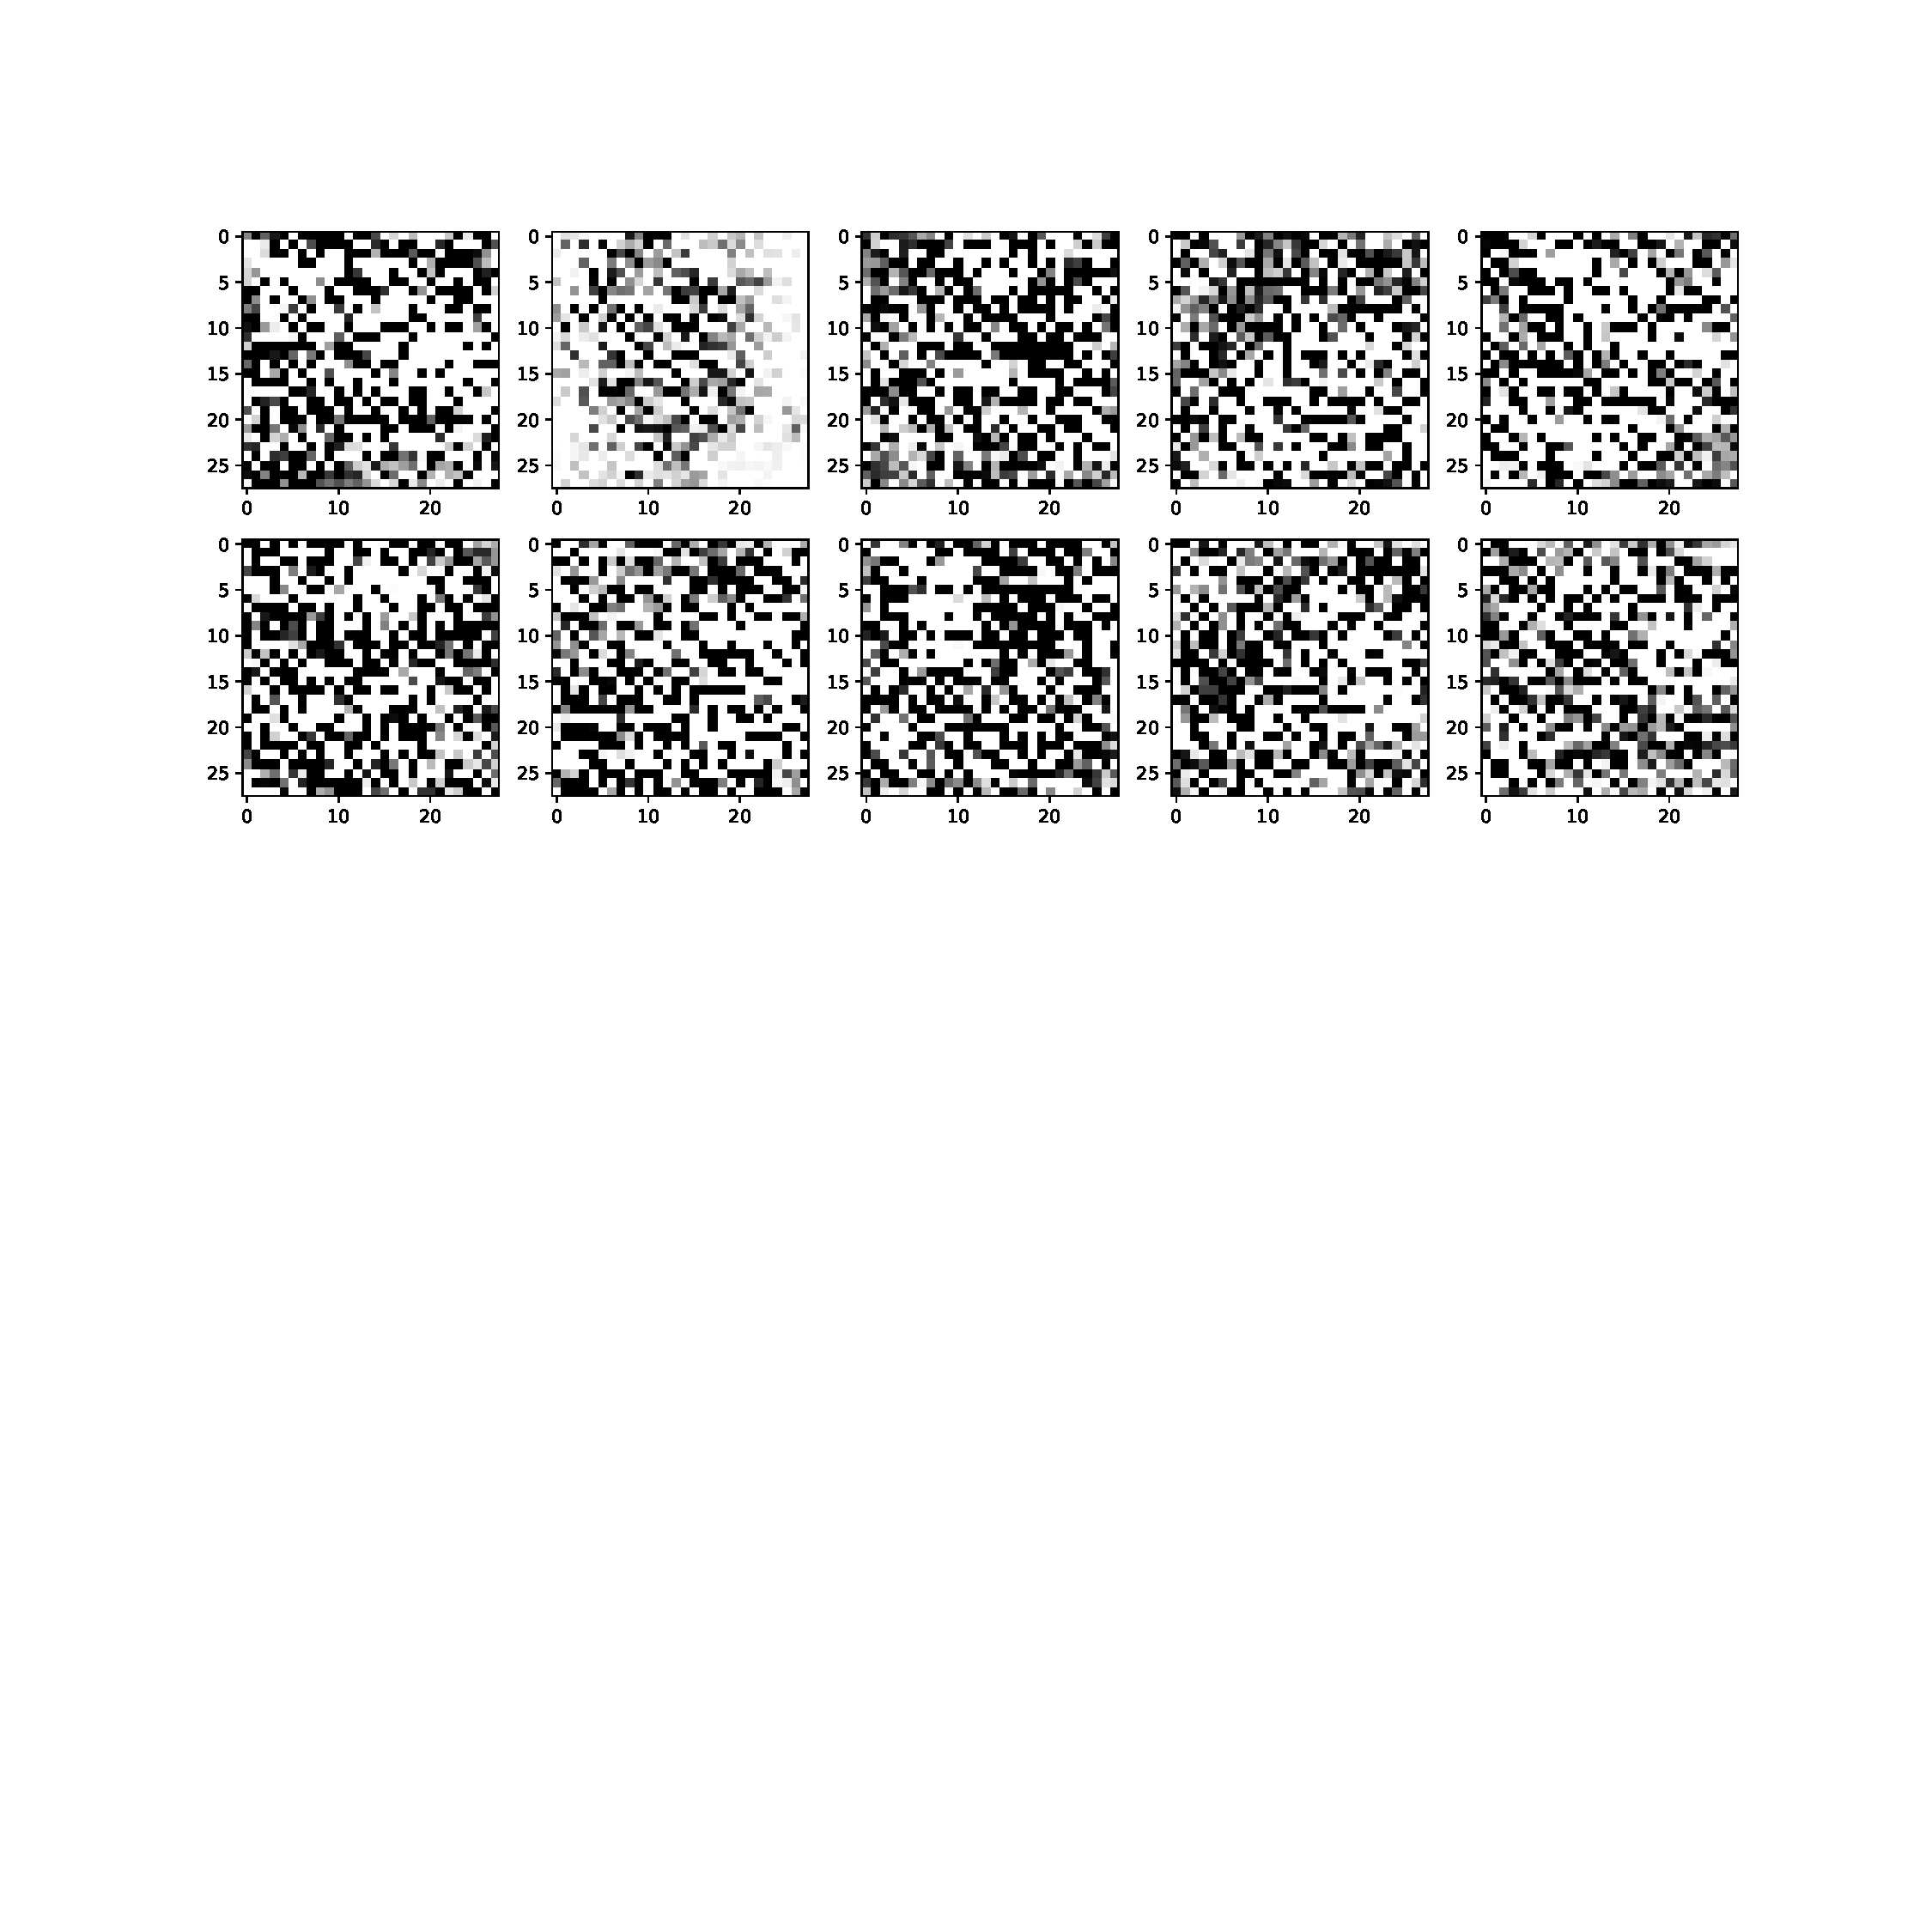
\includegraphics[width=\textwidth]{images/Native_attack/Mnistattack6.pdf}
         \vspace{-8em}
         \caption{SPML+Privacy; $\epsilon$=6 ; and, Accuracy=80.19\%}
         \label{default}
     \end{subfigure}
     \begin{subfigure}{.325\textwidth}
         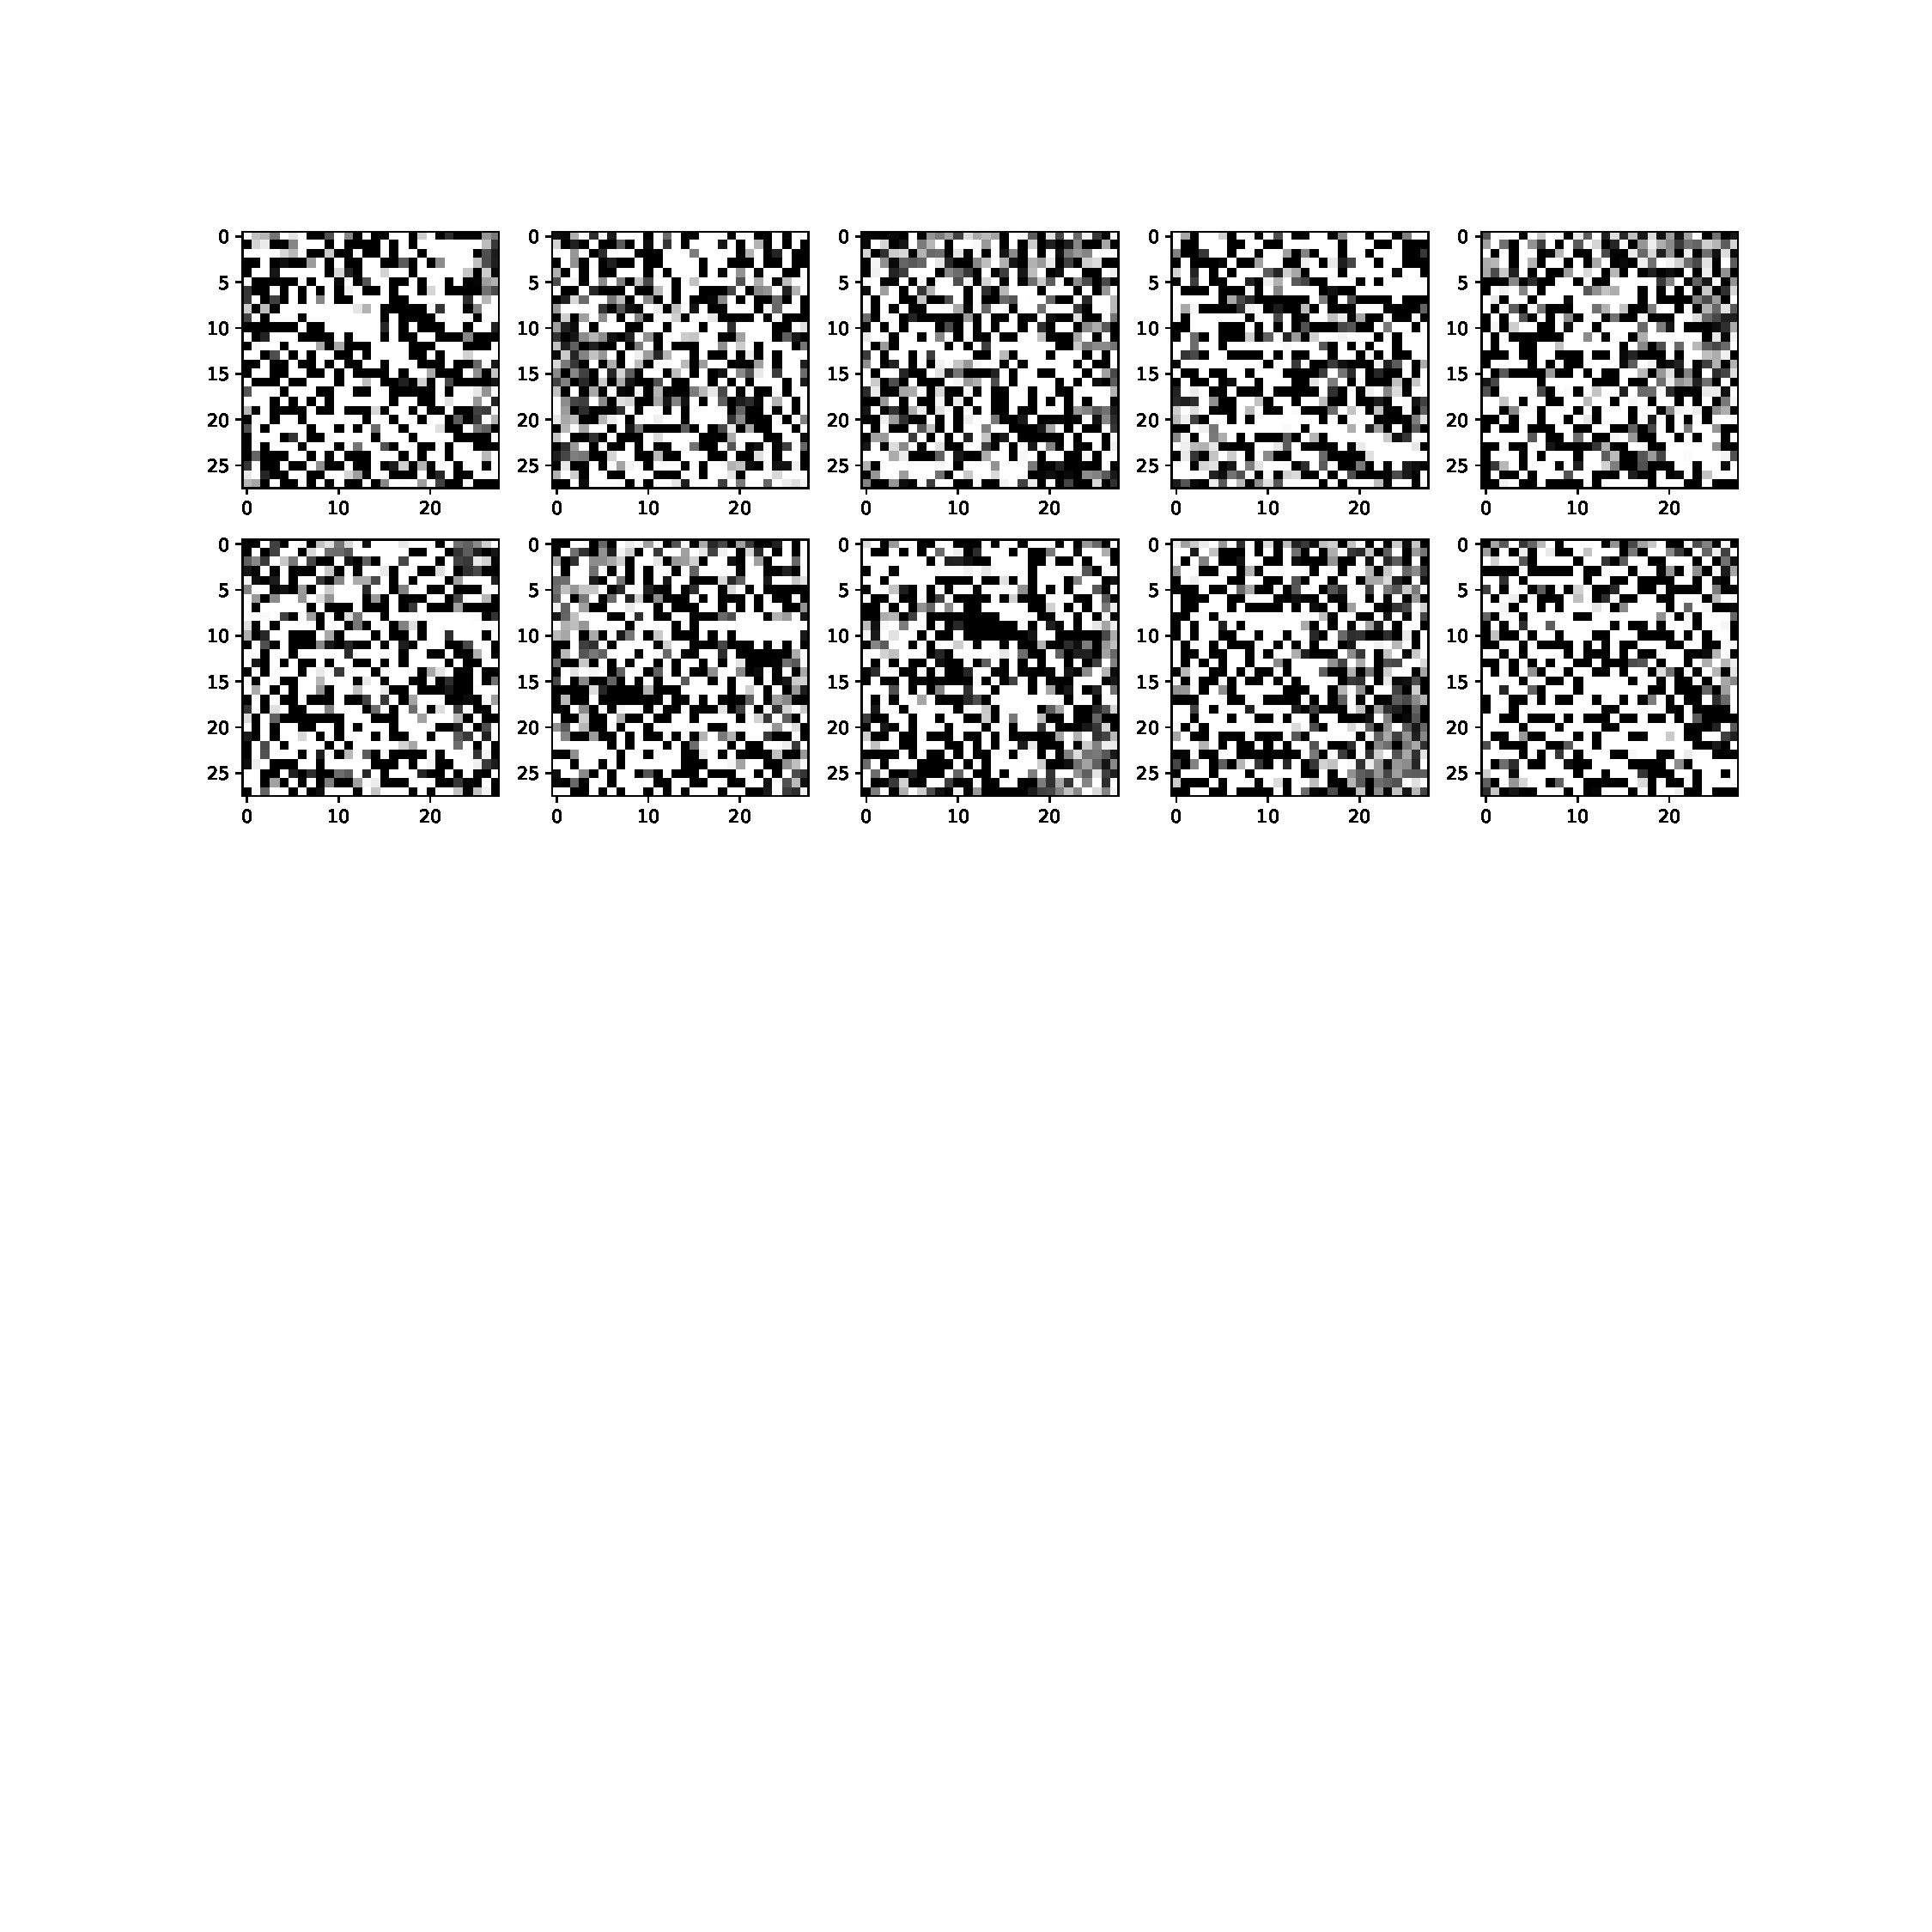
\includegraphics[width=\textwidth]{images/Native_attack/Mnistattack8.pdf}
         \vspace{-8em}
         \caption{SPML+Privacy; $\epsilon$=8 ; and, Accuracy=85.36\%}
         \label{default}
     \end{subfigure}
        \caption{Model inversion attack images - Native mode without Intel SGX and SCONE}
        \label{default}
\end{figure}

\begin{figure}
     \begin{subfigure}{.325\textwidth}
         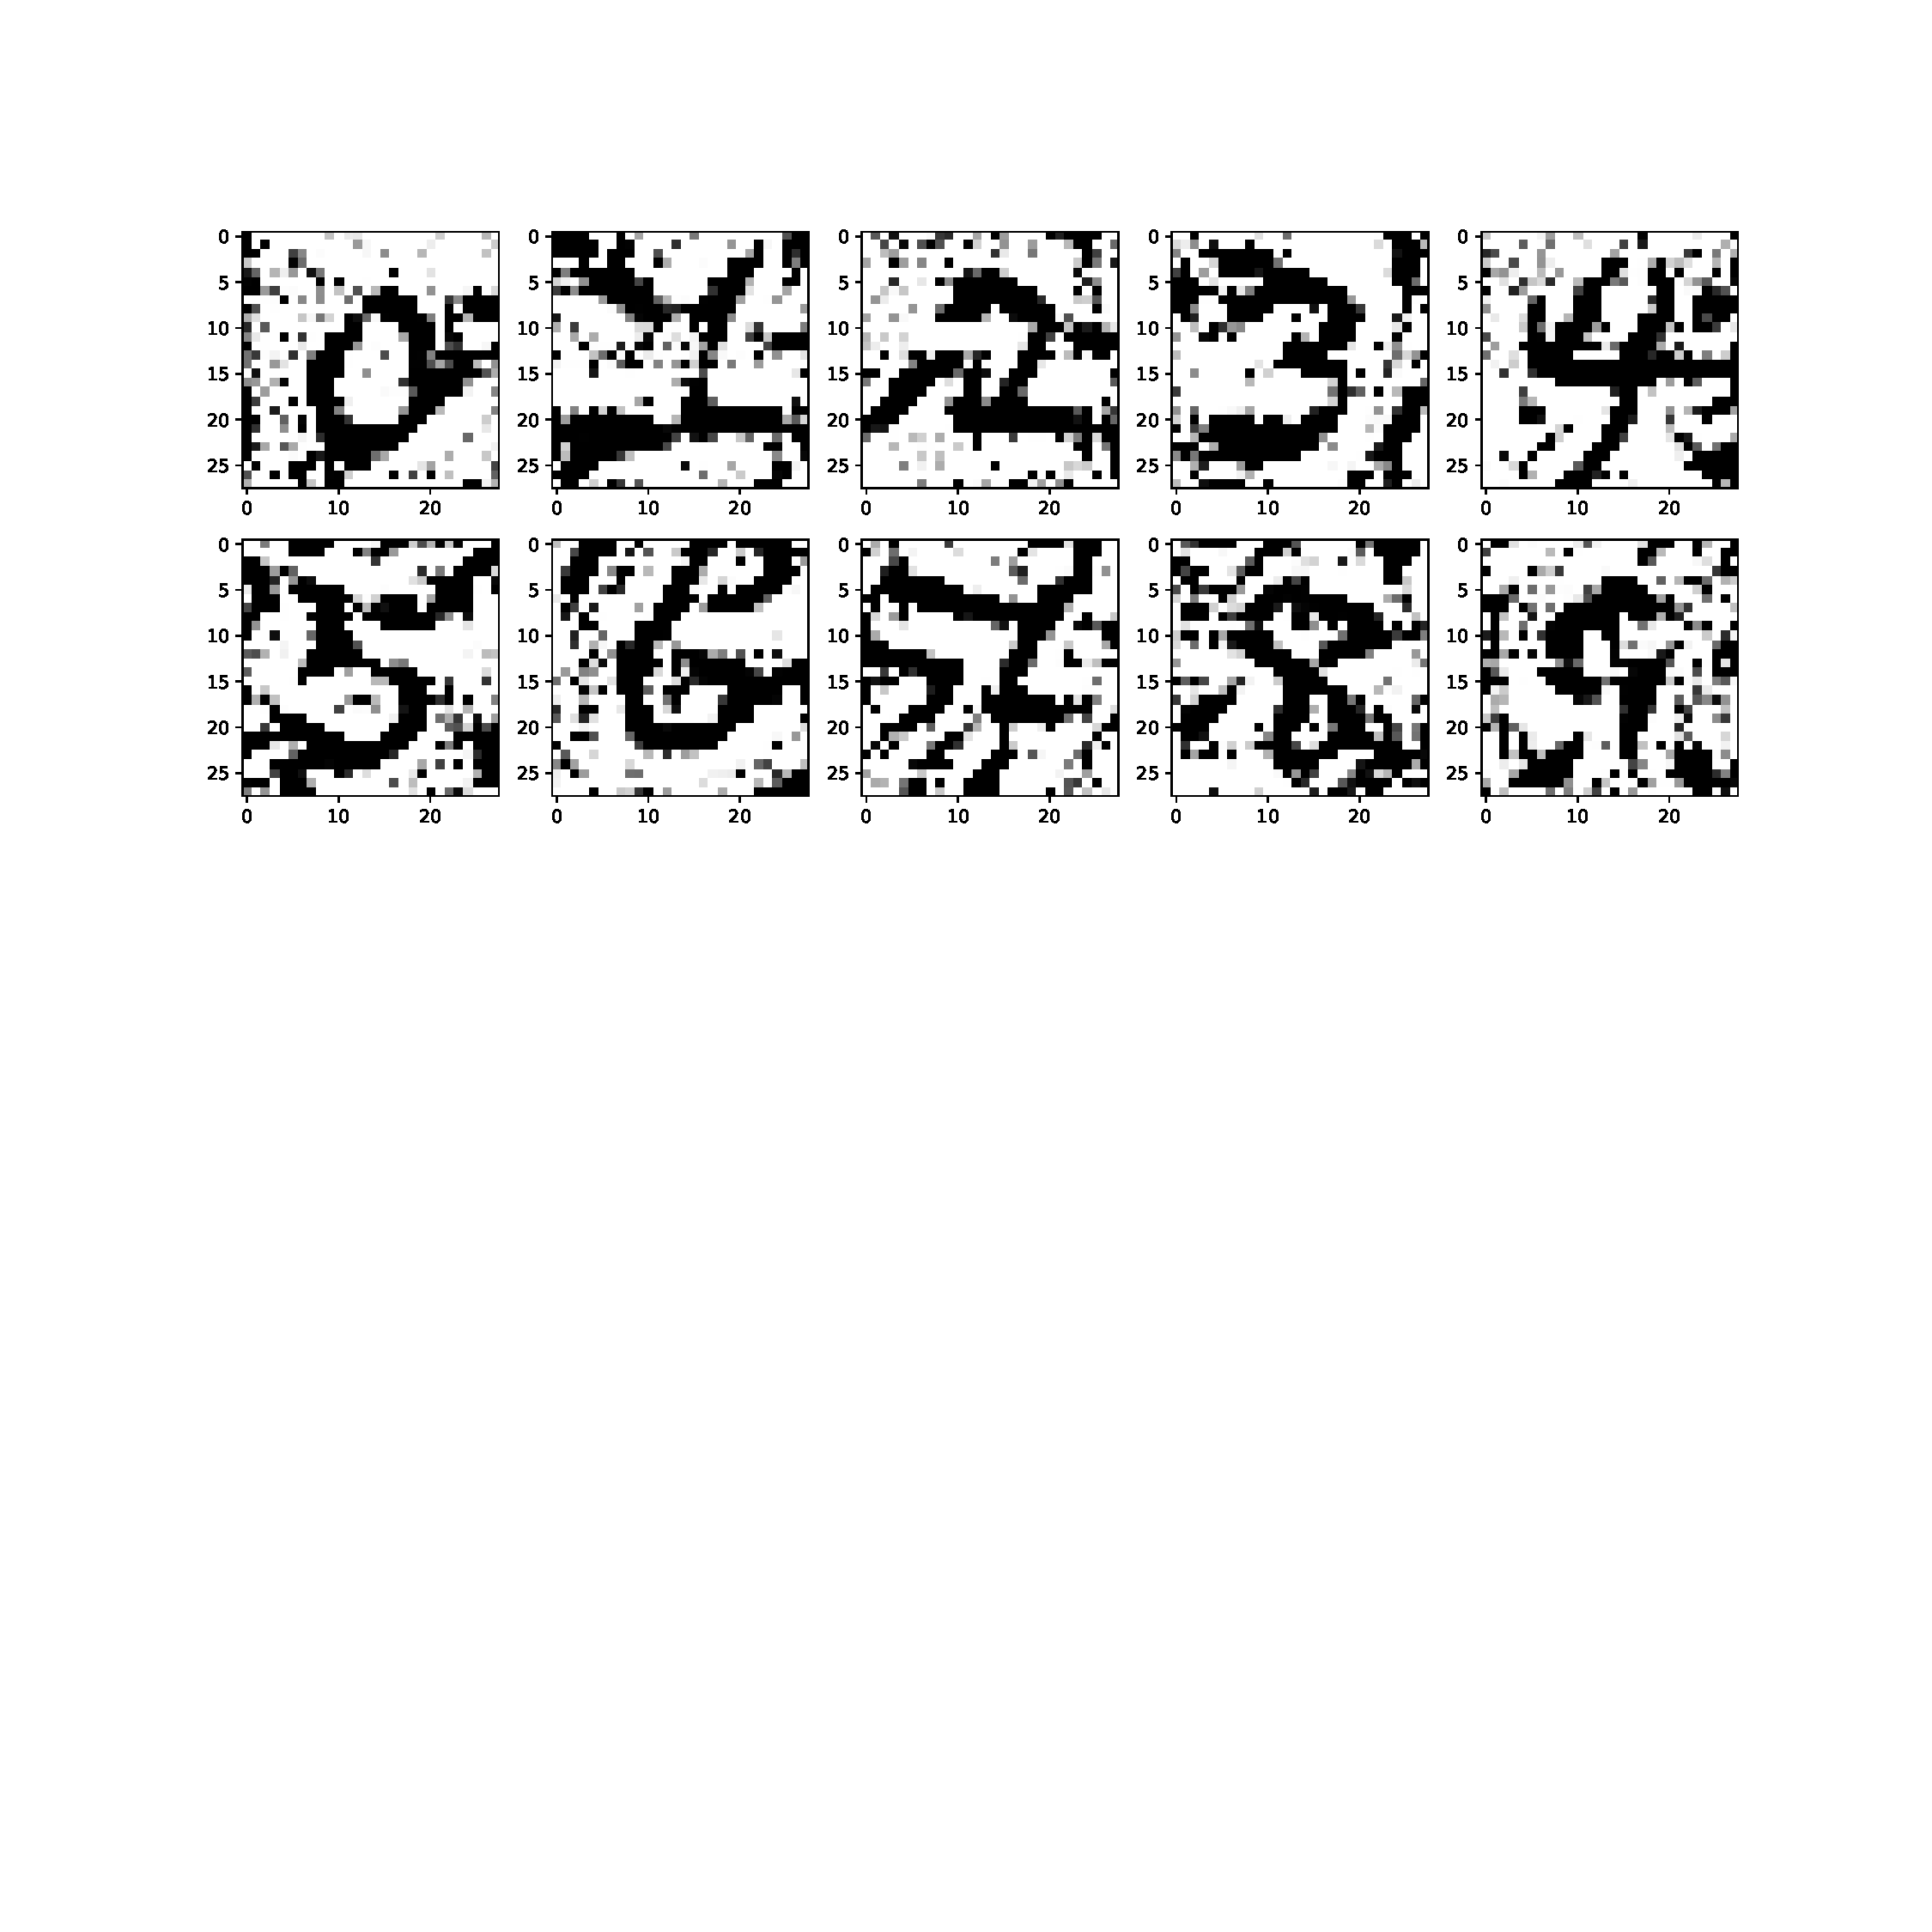
\includegraphics[width=\textwidth]{images/Sim_attack/Mnistattack_native.pdf}
         \vspace{-8em}
         \caption{SPML+Native TensorFlow; and, accuracy=99.72\%}
         \label{default}
     \end{subfigure}
     \begin{subfigure}{.325\textwidth}
         \includegraphics[width=\textwidth]{images/Sim_attack/Mnistattack.2.pdf}
         \vspace{-8em}
         \caption{SPML+Privacy; $\epsilon$=0.2; and, Accuracy=11.66\%}
         \label{default}
     \end{subfigure}
     \begin{subfigure}{.325\textwidth}
         \includegraphics[width=\textwidth]{images/Sim_attack/Mnistattack1.pdf}
         \vspace{-8em}
         \caption{SPML+Privacy; $\epsilon$=1; and, Accuracy=10.07\%}
         \label{default}
     \end{subfigure}
     \begin{subfigure}{.325\textwidth}
         \includegraphics[width=\textwidth]{images/Sim_attack/Mnistattack2.pdf}
         \vspace{-8em}
         \caption{SPML+Privacy; $\epsilon$=2; and, Accuracy=10.54\%}
         \label{default}
     \end{subfigure}
     \begin{subfigure}{.325\textwidth}
         \includegraphics[width=\textwidth]{images/Sim_attack/Mnistattack4.pdf}
         \vspace{-8em}
         \caption{SPML+Privacy; $\epsilon$=4; and, Accuracy=67.76\%}
         \label{default}
     \end{subfigure}
     \begin{subfigure}{.325\textwidth}
         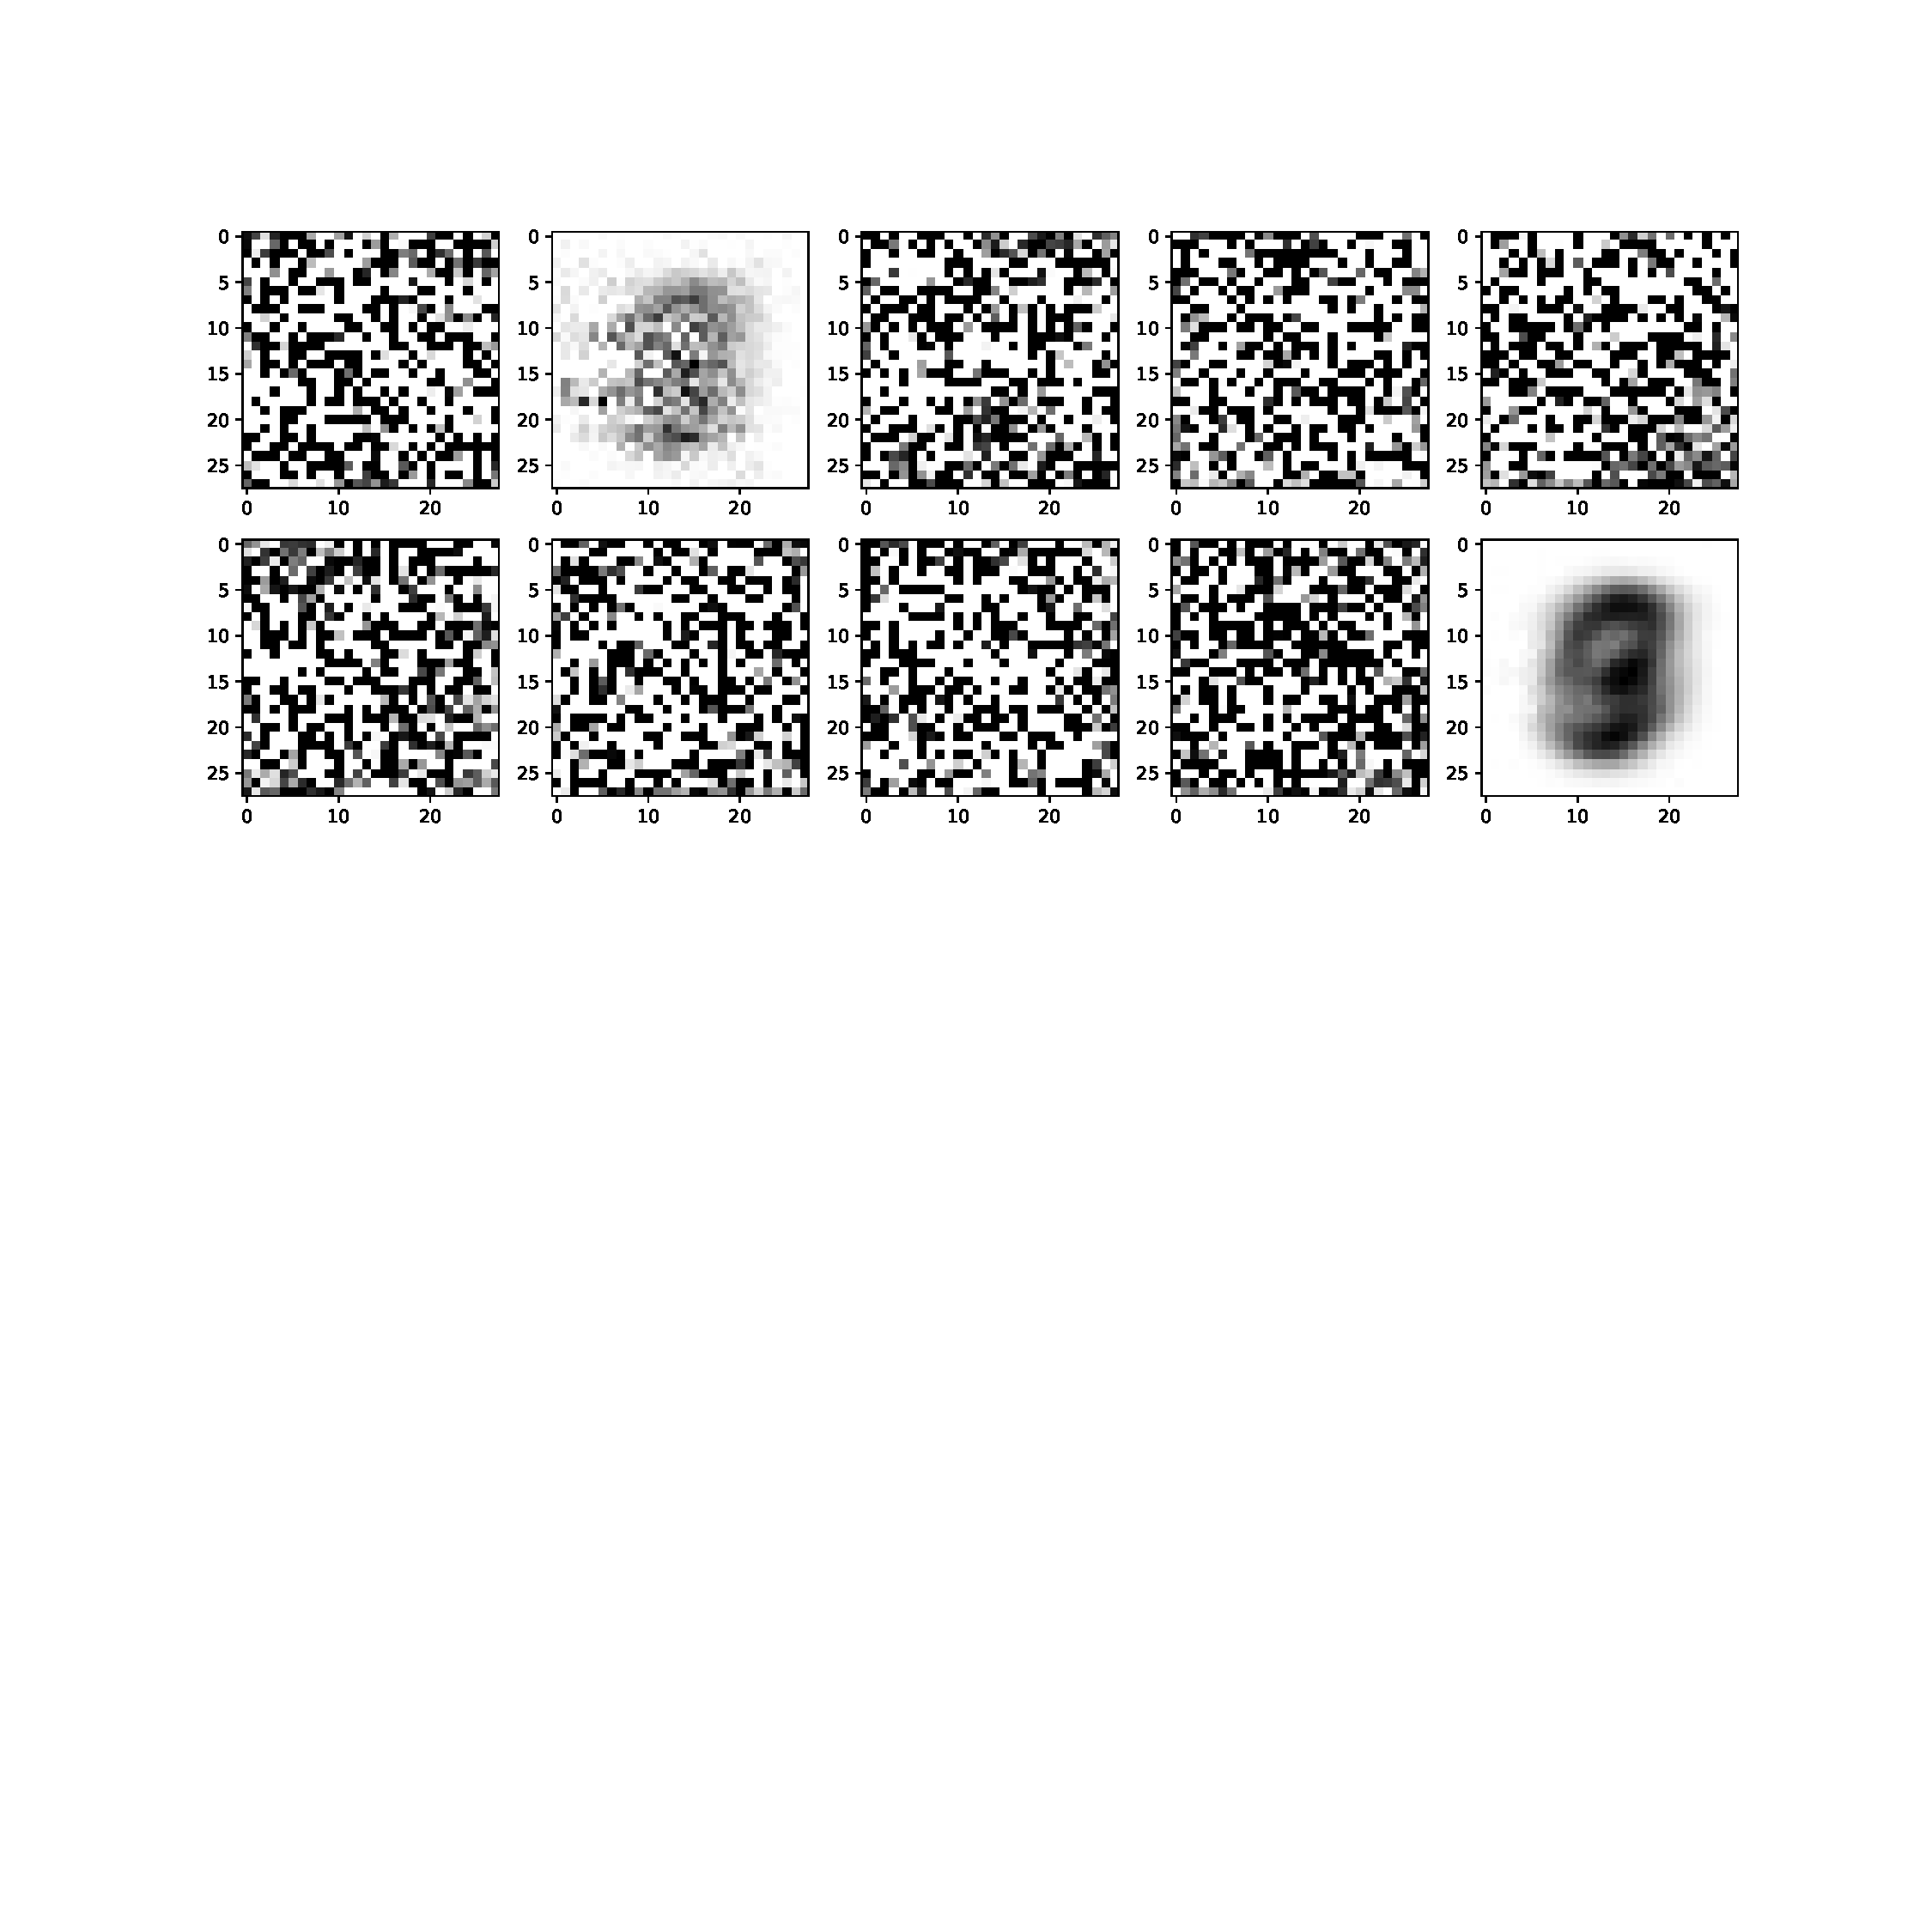
\includegraphics[width=\textwidth]{images/Sim_attack/Mnistattack6.pdf}
         \vspace{-8em}
         \caption{SPML+Privacy; $\epsilon$=6; and, Accuracy=71.6\%}
         \label{default}
     \end{subfigure}
     \begin{subfigure}{.325\textwidth}
         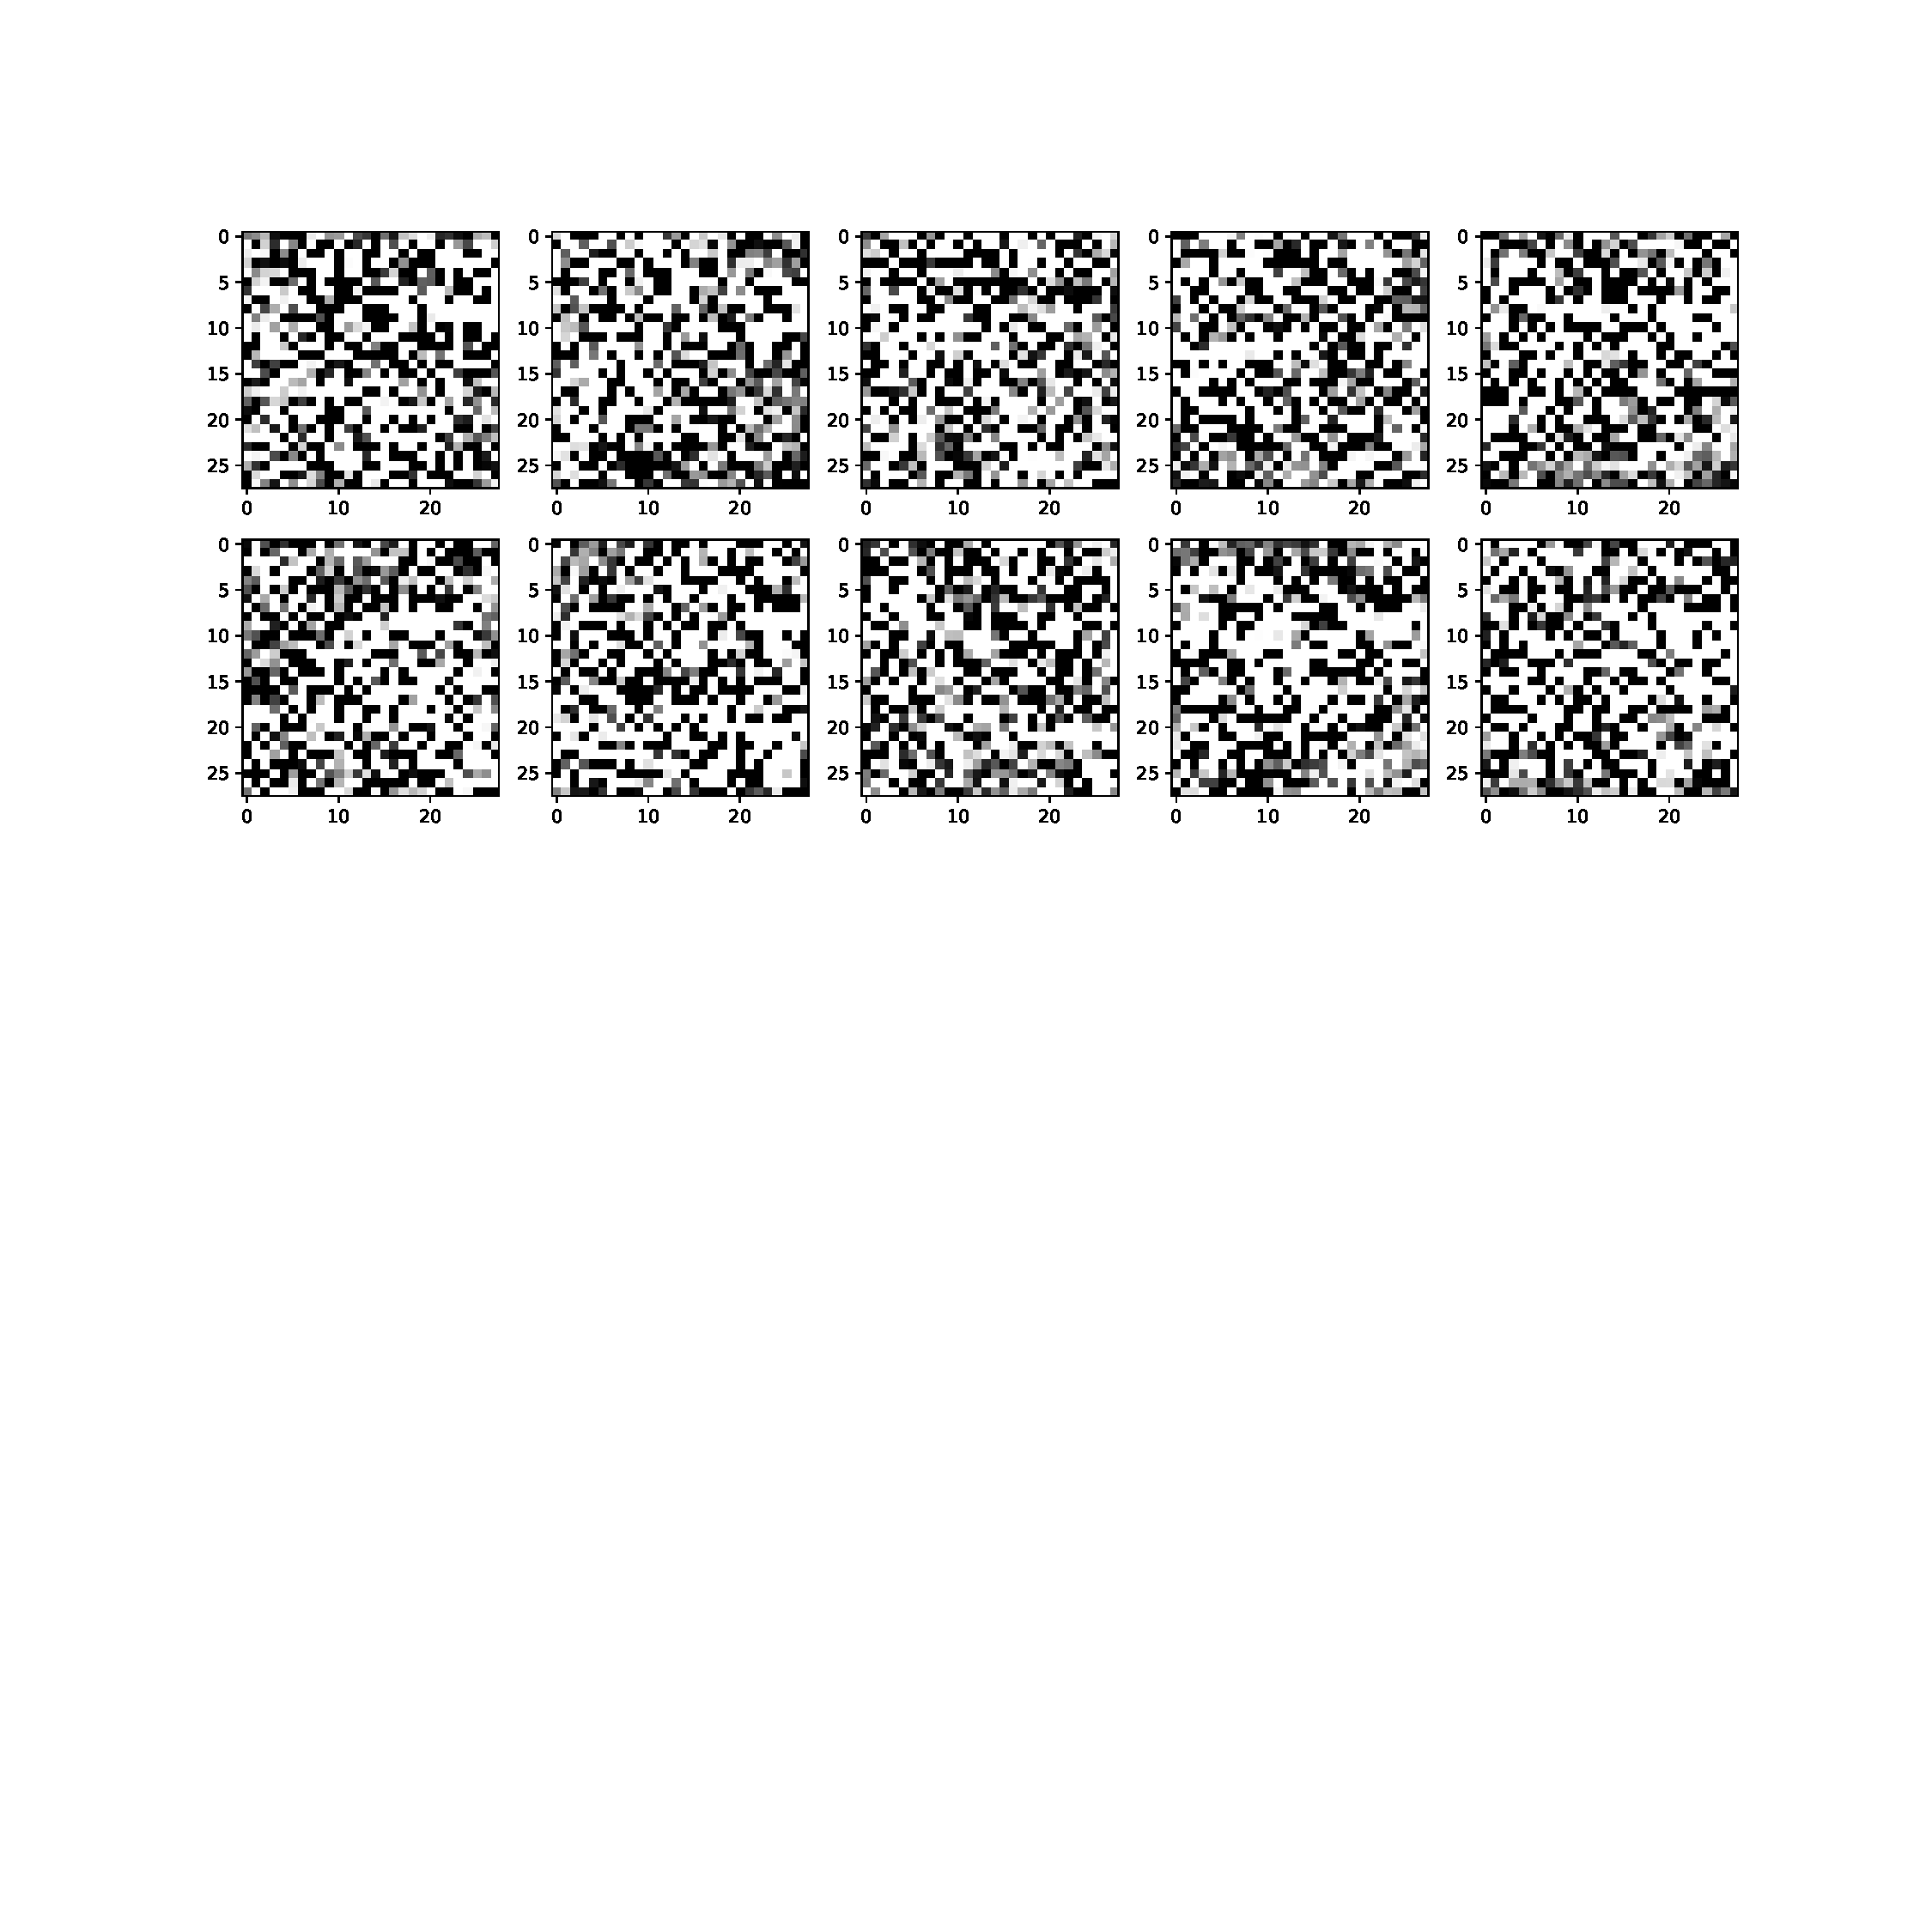
\includegraphics[width=\textwidth]{images/Sim_attack/Mnistattack8.pdf}
         \vspace{-8em}
         \caption{SPML+Privacy; $\epsilon$=8; and, Accuracy=84.37\%}
         \label{default}
     \end{subfigure}
        \caption{Model inversion attack images - SCONE simulation mode without Intel SGX and with SCONE}
        \label{default}
\end{figure}

\begin{figure}
     \begin{subfigure}{.325\textwidth}
         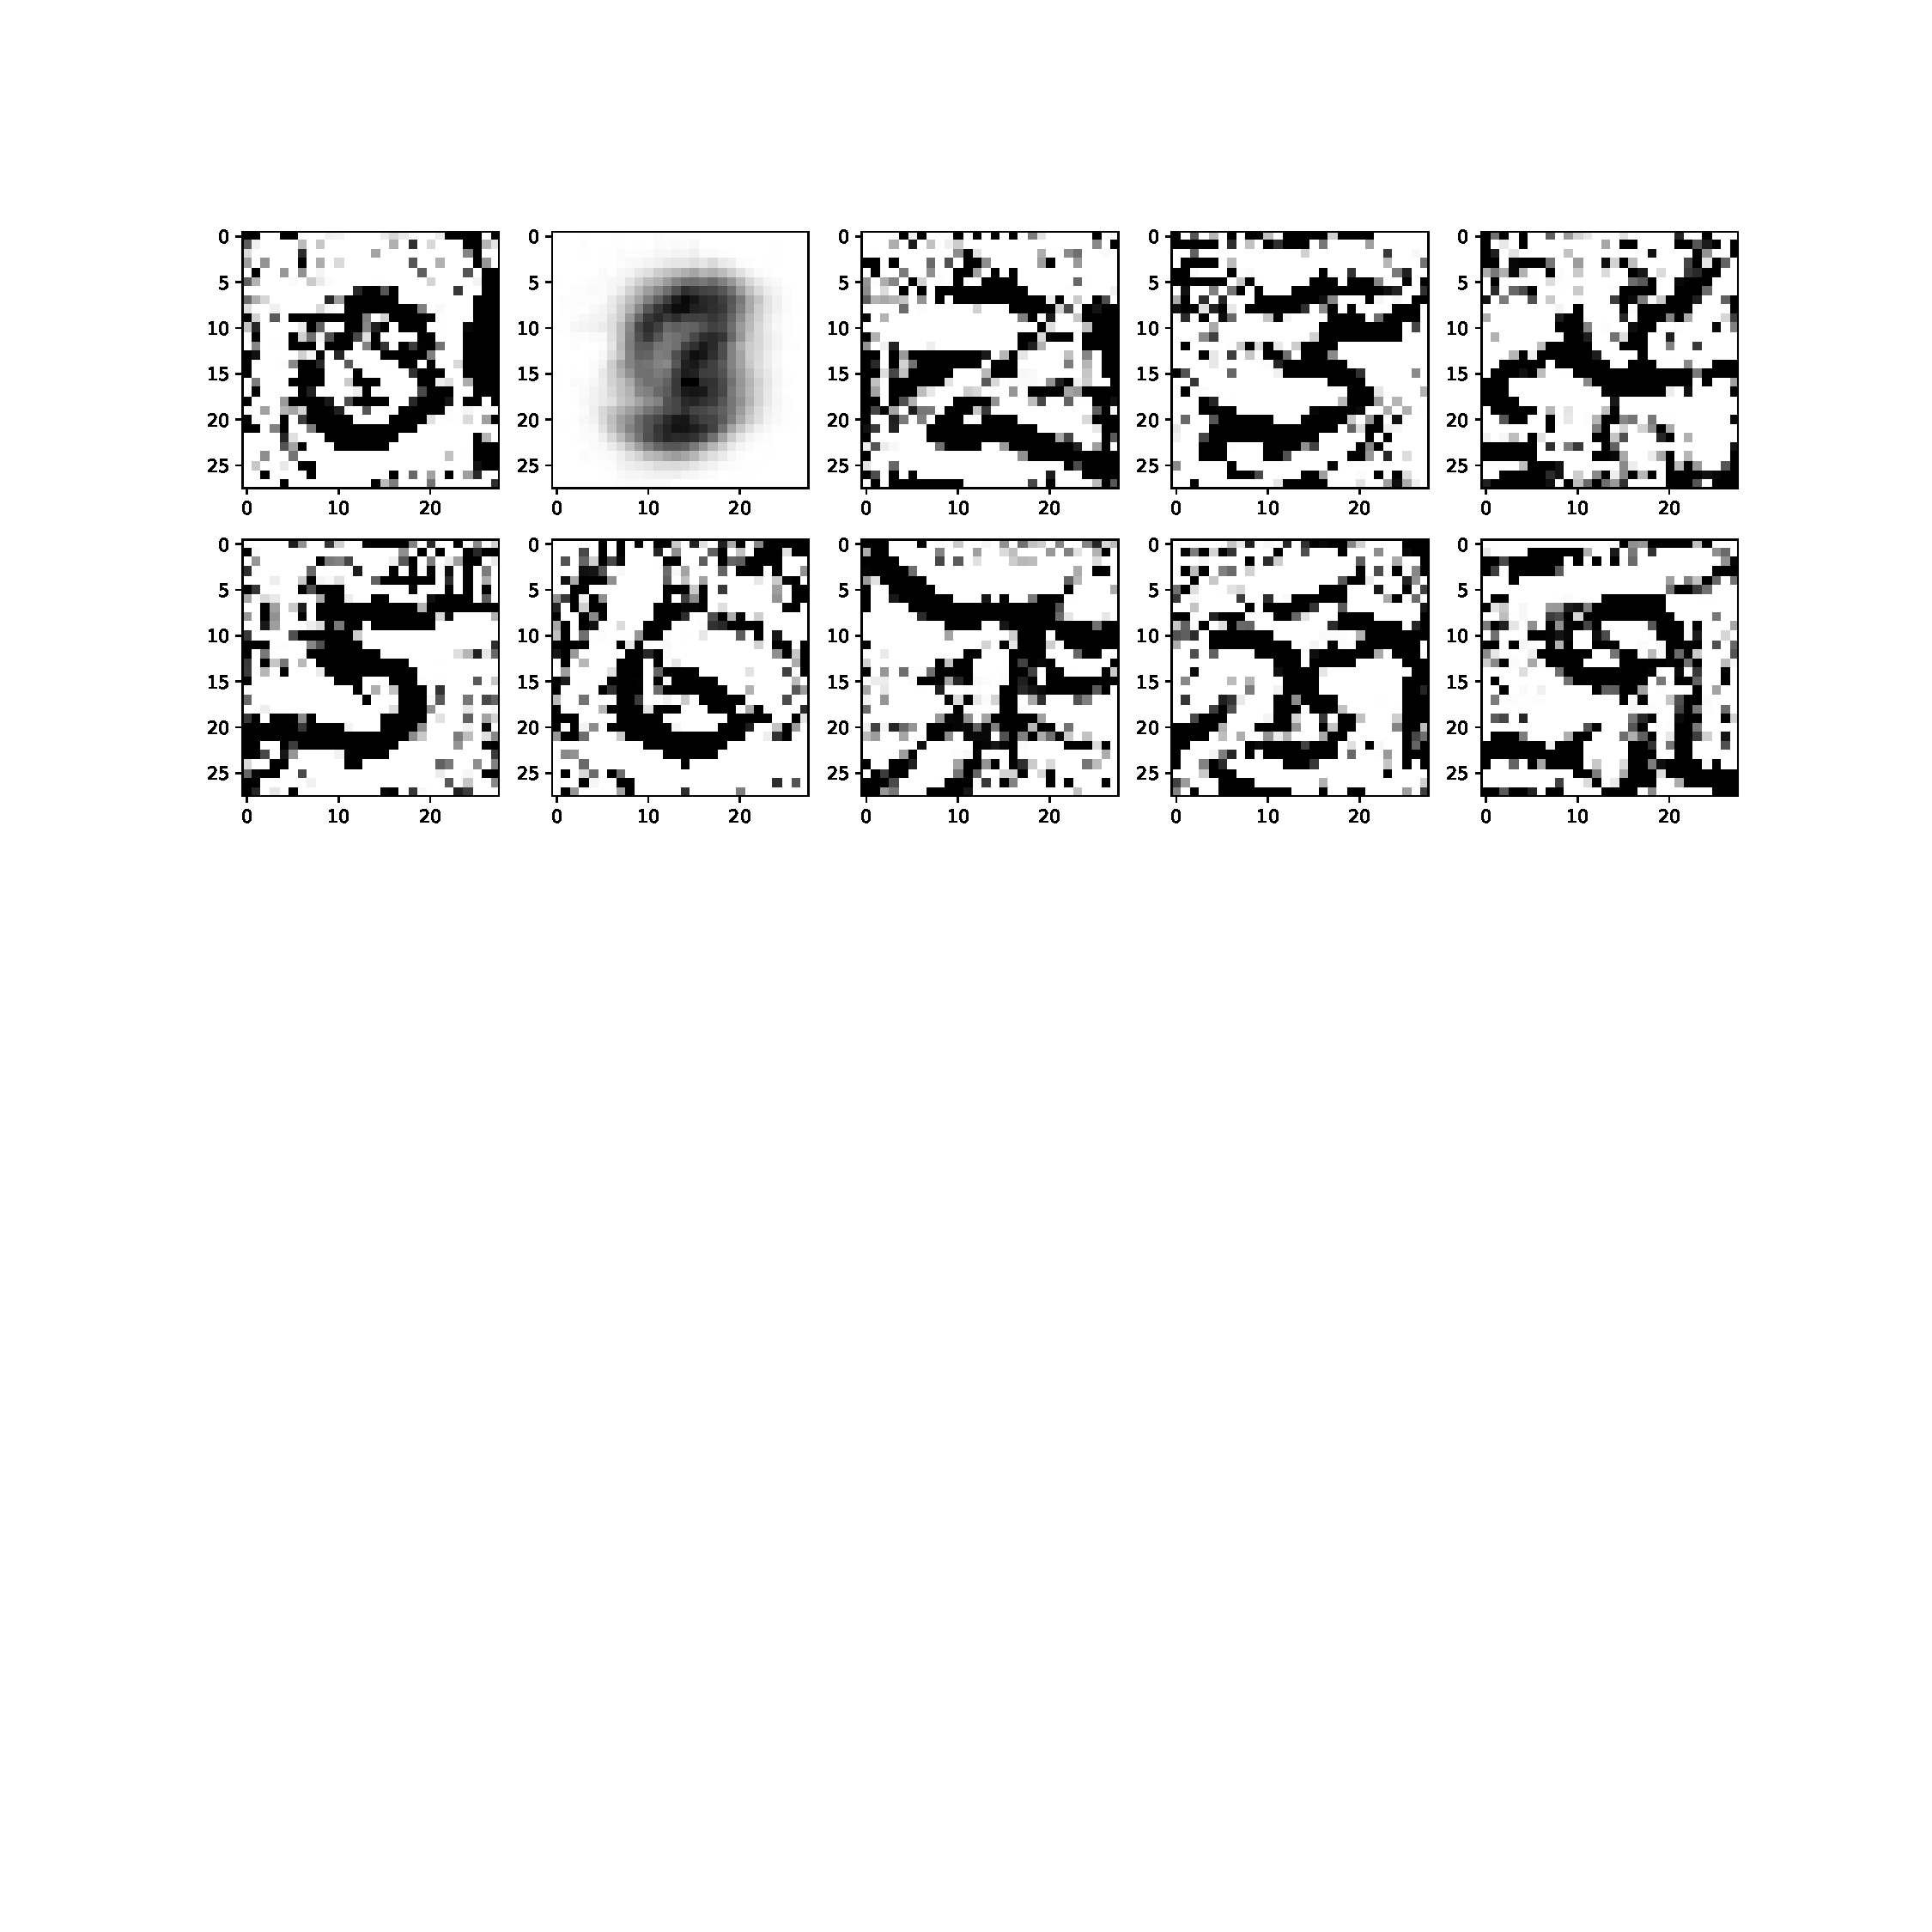
\includegraphics[width=\textwidth]{images/Hw_attack/Mnistattack_native.pdf}
         \vspace{-8em}
         \caption{SPML+Native TensorFlow; and, accuracy=99.65\%}
         \label{default}
     \end{subfigure}
     \begin{subfigure}{.325\textwidth}
         \includegraphics[width=\textwidth]{images/Hw_attack/Mnistattack.2.pdf}
         \vspace{-8em}
         \caption{SPML+Privacy; $\epsilon$=0.2; and, Accuracy=10.19\%}
         \label{default}
     \end{subfigure}
     \begin{subfigure}{.325\textwidth}
         \includegraphics[width=\textwidth]{images/Hw_attack/Mnistattack1.pdf}
         \vspace{-8em}
         \caption{SPML+Privacy; $\epsilon$=1; and, Accuracy=10.13\%}
         \label{default}
     \end{subfigure}
     \begin{subfigure}{.325\textwidth}
         \includegraphics[width=\textwidth]{images/Hw_attack/Mnistattack2.pdf}
         \vspace{-8em}
         \caption{SPML+Privacy; $\epsilon$=2; and, Accuracy=10.39\%}
         \label{default}
     \end{subfigure}
     \begin{subfigure}{.325\textwidth}
         \includegraphics[width=\textwidth]{images/Hw_attack/Mnistattack4.pdf}
         \vspace{-8em}
         \caption{SPML+Privacy; $\epsilon$=4; and, Accuracy=53.13\%}
         \label{default}
     \end{subfigure}
     \begin{subfigure}{.325\textwidth}
         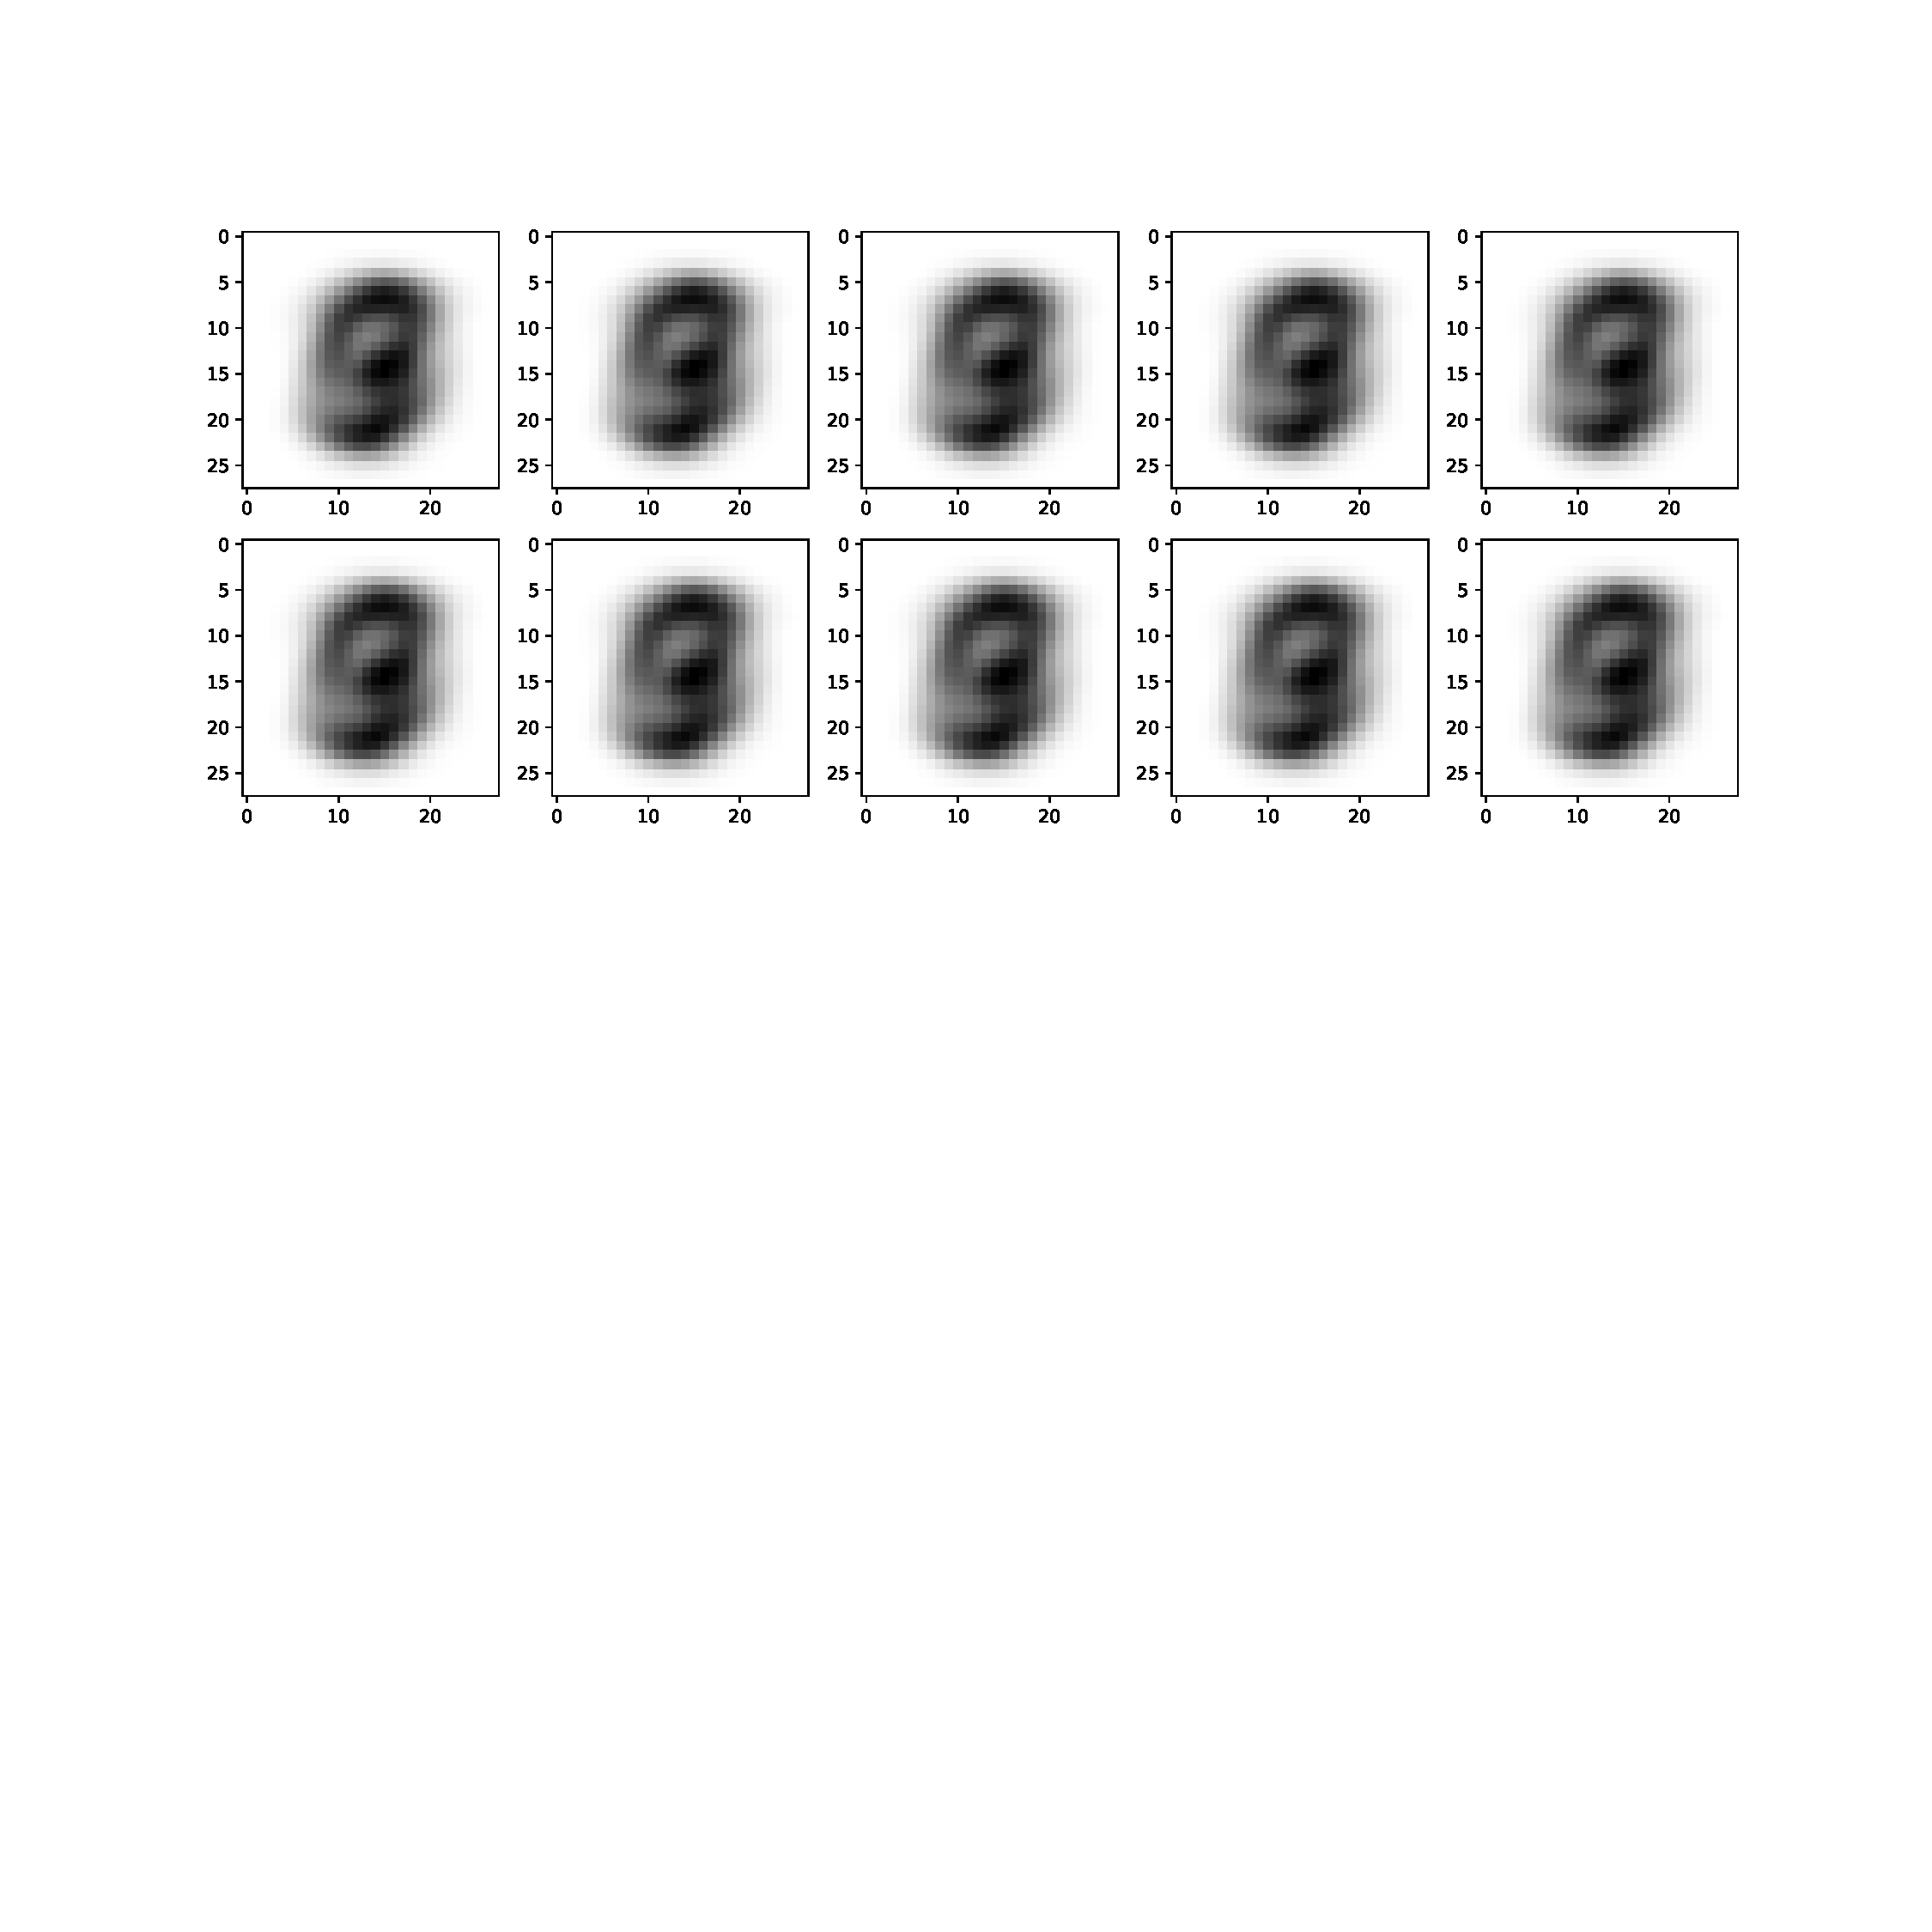
\includegraphics[width=\textwidth]{images/Hw_attack/Mnistattack6.pdf}
         \vspace{-8em}
         \caption{SPML+Privacy; $\epsilon$=6; and, Accuracy=75.92\%}
         \label{default}
     \end{subfigure}
     \begin{subfigure}{.325\textwidth}
         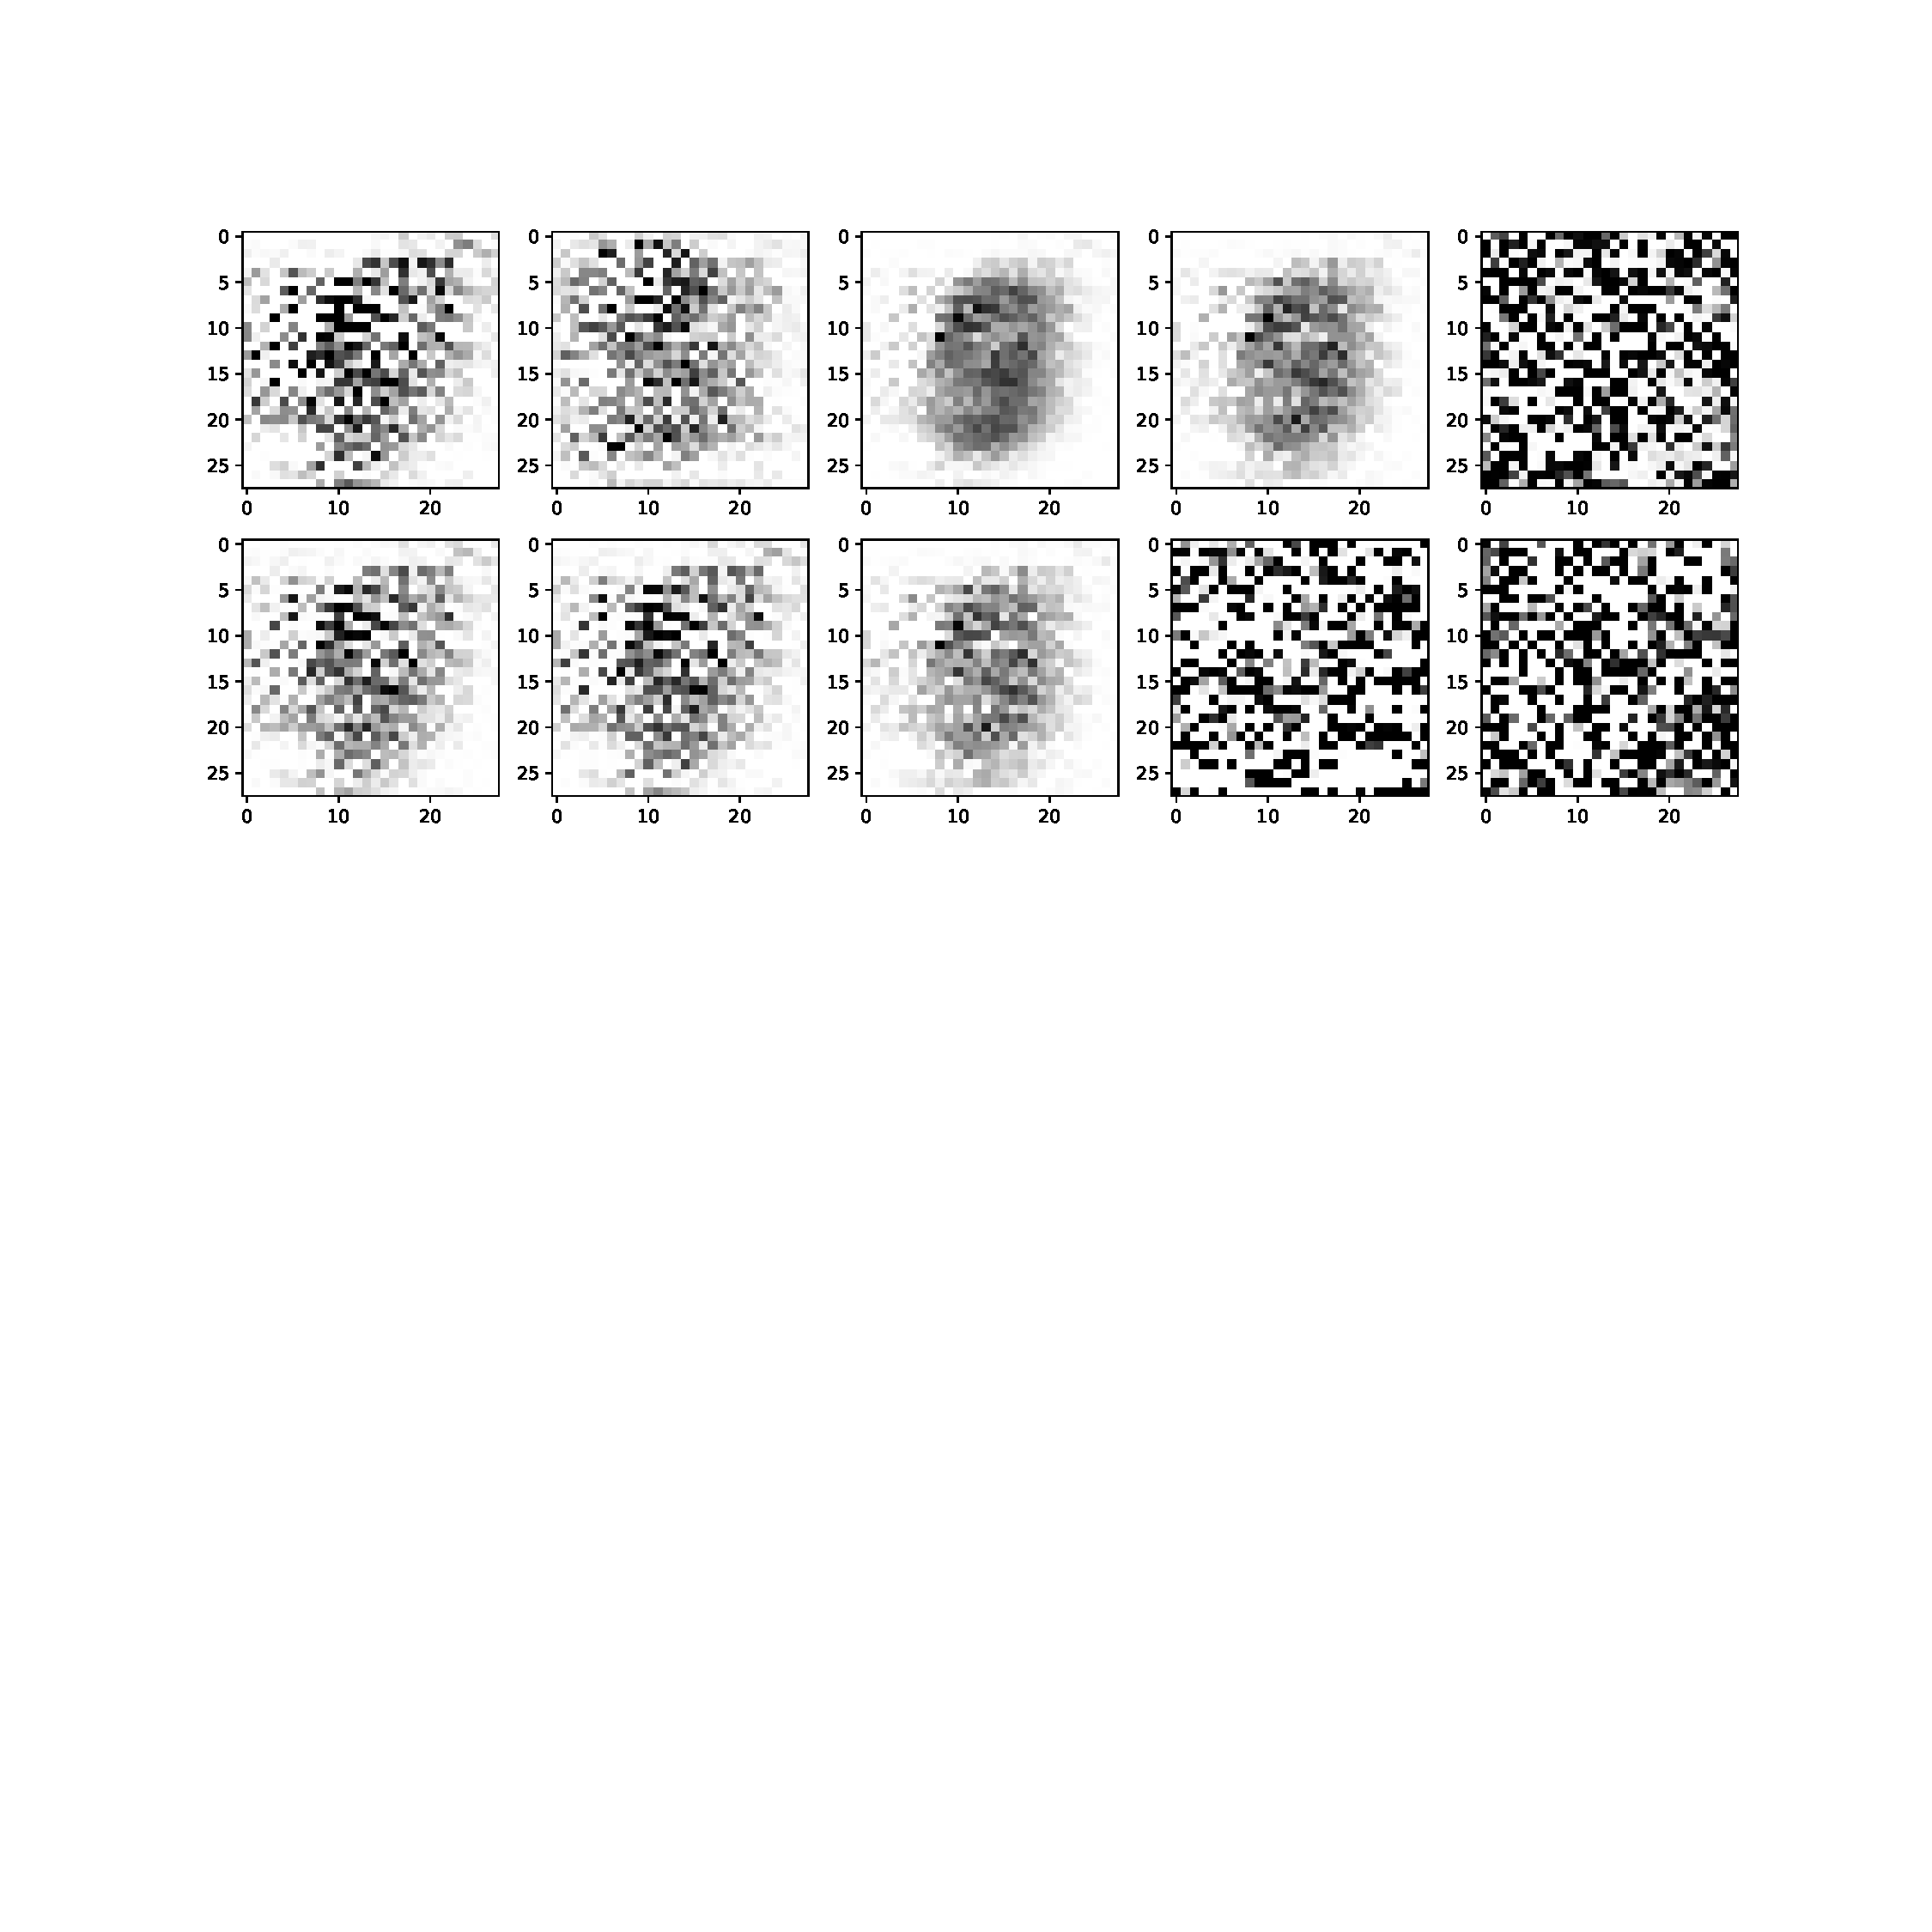
\includegraphics[width=\textwidth]{images/Hw_attack/Mnistattack8.pdf}
         \vspace{-8em}
         \caption{SPML+Privacy; $\epsilon$=8; and, Accuracy=85.93\%}
         \label{default}
     \end{subfigure}
        \caption{Model inversion attack images - SCONE hardware mode with Intel SGX and with SCONE}
        \label{default}
\end{figure}